\chapter{Control-Flow-Driven Verification}\label{ch:cfg}

\section{Introduction}\label{se:cfg_intro}
The memory usage analysis approach presented in this chapter
features a Floyd-style methodology as described in \cref{se:cfg_invariant}.
This methodology allows for minimization of symbolic execution
\index{symbolic execution} while still ensuring correctness.
It also provides proper loop handling.
An overview of the methodology can be seen in \cref{fig:cfg_overview}.

The main goal of the approach is to prove the property of \emph{memory preservation},
\index{memory!preservation}
fully described in \cref{se:memory_preservation}.
In short, this property ensures only documented regions of memory are modified;
\index{memory!region}
anything outside of those regions remains unchanged.
This property has the potential to be used
to prove the absence of common memory-related issues,
such as buffer overflows or some forms of data leakage.

To achieve minimal symbolic execution,
it features automatically-selected cutpoints obtained via control flow analysis
\index{cutpoint}
using the tool angr~\citep{shoshitaishvili2016state}.
\index{angr}
The cutpoints are described in \cref{se:cfg_invariant}.
Basic starting predicates for those preconditions and postconditions
as well as the cutpoints are generated,
but the bulk of the information must be added manually.
Larger-scale scalability is achieved by using function-level compositionality.
Recursion is supported but requires a significant amount of work,
much greater than that needed for loops and function calls alone.
\index{loop}
\index{function!call}

\tikzstyle{myblock} = [rectangle, draw, text width=2.25cm, text centered, rounded corners, minimum height=2cm]
\begin{figure}
  \centering
  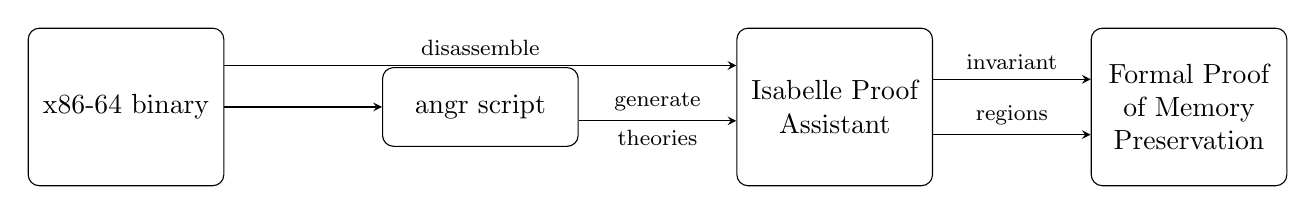
\begin{tikzpicture}[node distance=4.5cm, auto, >=stealth, ->]
  \node [myblock] (binary) {x86-64 binary};
  \node [myblock, right of=binary, minimum height=1cm] (cfg) {angr script};
  \node [myblock, right of=cfg] (isa) {Isabelle Proof Assistant};
  \node [myblock, right of=isa] (mem) {Formal Proof of Memory Preservation};
  \draw [transform canvas={yshift=1.5em}] (binary) -- node[above] {\footnotesize disassemble} (isa);
  \draw (binary) -- (cfg);
  \draw [transform canvas={yshift=-.5em}] (cfg) -- node[above] {\footnotesize generate} node[below] {\footnotesize theories}(isa);
  \draw [transform canvas={yshift=1em}] (isa) -- node[above] {\footnotesize invariant} (mem);
  \draw [transform canvas={yshift=-1em}] (isa) -- node[above] {\footnotesize regions} (mem);
  \end{tikzpicture}
  \caption{Overview of Methodology}\label{fig:cfg_overview}
\end{figure}

The methodology was applied to several example functions
as well as to functions
from the HermitCore unikernel library~\citep{lankes2016hermitcore}.
\index{HermitCore}
\index{unikernel}
HermitCore is \iac{os} kernel library aiming to provide real-time guarantees for high-performance computing.
Documentation of the example functions can be found in \cref{se:cfg_examples},
while the HermitCore function work can be found in \cref{se:cfg_application}.
These functions have a variety of features such as loops,
non-trivial data structures, pointers, subcalls, and even recursion in some cases.

% TODO: maybe move into Memory Usage section
\section{Memory Preservation}\label{se:memory_preservation}
Memory preservation shows that the values written by a program
\index{memory!preservation}
are restrained to specified regions in memory.
Those regions cannot be fully identified when working with source code alone,
particularly when the end result is optimized.
Memory may be laid out differently depending on the \ac{isa} and \ac{abi} targeted,
as well as on the compiler used.
This can include positioning of global variables as well as the layout of stack frames.
\index{stack!frame}
While one way of resolving that issue would be to choose a specific compiler
and provide a formal analysis of how it arranges memory, that method is not flexible.
It may instead be better to target assembly or machine code directly,
as done in this dissertation.

\subsection{Usefulness}
The following small sections elaborate on the usefulness of memory preservation
as a platform for further verification efforts.

\subsubsection{Security}
Unbounded memory usage can lead to vulnerabilities
such as buffer overflows and data leakage.
One example of such a vulnerability would be 2014's Heartbleed~\citep{heartbleed}.
Heartbleed was caused by a lack of bounds checking on a string array
requested as output as part of a ``heartbeat'' message.
This, combined with a custom memory manager
that also had no security protections against out-of-bounds memory accesses,
lead to potential leakage of sensitive data such as passwords and encryption keys.
% TODO: need another, better example that involves data modification too
Memory preservation can serve as a foundation for formal security analyses
\index{memory!preservation}
that could be used to expose vulnerabilities involving malicious writes.

\subsubsection{Composition}
Scalability in verification is only feasible with composition.
Proofs of functional correctness over a large suite of software
require decomposing that suite into manageable chunks.
Separation logic provides a \emph{frame rule} that supports such decomposition\cite{reynolds2002separation}.
In words, the frame rule states that,
if a program or program fragment can be confined to a certain part of a state,
properties of that program or program fragment carry over
when used as part of a larger system involving that state.
Memory preservation allows for discharging the most involved part of the frame rule,
at least in terms of individual assembly functions.
That is, it shows that the memory usage of those functions is constrained
to specific regions in memory.
This can then serve as a basis
for any larger proof effort over multifunction assembly programs.

\subsubsection{Concurrency}
Reasoning over concurrent programs is complicated
due to the potential interactions between threads.
While there are ways of handling such interactions in a structured manner
via kernel- or library-provided \ac{ipc},
one method commonly used for the sake of efficiency is \emph{shared memory}.
Shared memory, in the context of this work,
refers to threads or processes sharing either a full memory space
or portions of one (via memory mapping)
that can be written to and read from freely by any thread or process with access to it.
Usage of shared memory can result in \emph{unintended} interactions between threads.
Memory preservation could be adapted to show the absence of such interactions
by proving that multiple threads only write
to specifically-allowed regions of shared memory.
Doing so would, of course, require a proper model of concurrency,
which is out of scope of this dissertation.

\subsection{Formal Definition}
The formal definition of memory preservation starts with the notion of \emph{state}.
%TODO

\section{Floyd Invariant Foundation}\label{se:cfg_invariant}
% TODO: more here?

Loops pose a significant problem when using symbolic execution to analyze code.
\index{loop}
One of the major issues is that they result in significant path explosion.
While there are methodologies to reduce the number of paths to execute
when using loops~\citep{saxena2009lese,obdrzalek2011efficient},
those methods are not currently formally verified
and therefore not usable within Isabelle/HOL.
\index{Isabelle/HOL}
Additionally, deciding the loop condition on a symbolic state
may involve non-determinism (such as an event loop dependent on user input to exit),
\index{non-determinism}
which can cause infinite execution.

Breaking up symbolic execution of loops is one method of resolving those issues.
With the right annotations,
it is possible to only need to symbolically execute one iteration per loop.
This eliminates the above-mentioned loop issues.
That breaking up of loops can be accomplished using a control-flow-based approach
akin to \emph{Floyd verification}~\citep{floyd1967assigning}.
\index{Floyd!verification}
A state predicate assigned to an instruction within a loop
\index{state!predicate}
functions as an \emph{invariant} for that loop.
\index{loop!invariant}
Such invariants hold for every iteration of the loop,
allowing a symbolic description of the loop's behavior.
When combined with a general methodology
of structured preconditions and postconditions that show,
for each annotated state, the succeeding annotated state satisfies its state predicate,
a Hoare triple can be inferred for the program as a whole.
\index{Hoare!triple}

Taking this approach also allows minimizing symbolic execution
even in non-loop situations.
Consider the following pseudocode,
which sequentially executes an if-statement and some program~$P$:
\begin{flushleft}
  \texttt{if} $b$ \texttt{then} $x$ \texttt{else} $y$; $P$
\end{flushleft}
The assembly corresponding to this code can be verified using symbolic execution.
If executed in full, the symbolic execution engine
would require first considering the case where~$b$ is true,
executing~$x$ and subsequently symbolically executing program~$P$.
It would then consider the case where~$b$ is false, executing~$y$ followed by~$P$.
Program~$P$ would thus be symbolically executed twice.
This repetition can be avoided
by placing a cutpoint at the start of each block where control flow converges,
\index{cutpoint}
resulting in all instructions being symbolically executed only once each.
Each cutpoint, however, requires a state predicate contained
in a \emph{Floyd invariant}.
\index{Floyd!invariant}

The Floyd invariant for a function is a partial function
that take the form $I:L\rightharpoonup(S\mapsto\mathbb{B})$.%
\nomenclature{$L$}{The type of instruction addresses in a program; a 64-bit word}%
\nomenclature{$\mathbb{B}$}{The type of boolean values, True and False}
This function maps from instruction addresses with invariants
to the corresponding state predicate that is the invariant.
As a technical detail, some function proofs require additional arguments to $I$
that represent the arguments passed to the function.
\begin{definition}
  A Floyd invariant~$I$ \emph{holds} if and only if, for any state~$\sigma$,
  \begin{equation}
    I(\loc\sigma)(\sigma)\longrightarrow
    \sigma'\neq\bot_E\wedge(\sigma'=\bot_{\var{NT}}\vee I(\loc\sigma')(\sigma')),
  \end{equation}%
  \nomenclature{$\bot_\var{NT}$}{Indicates non-termination}
  where
  $\sigma'=\run((\lambda\sigma\cdot I(\loc\sigma)(\sigma)\neq\bot),\sigma)$%
  \nomenclature{$\bot$}{Used here to represent the result of calling a partial function with a value it does not have an actual result for}
  and $\loc\sigma$ is the current program location,
  stored in \inlineasm{rip} on x86-64 systems.
\end{definition}
In words, if the Floyd invariant holds on the current state~$\sigma$,
then running to the next annotated location does not produce an exception.
If it terminates, the produced state~$\sigma'$ satisfies the Floyd invariant.

The following theorem states that a Floyd invariant
can be used to prove properties over its corresponding program or function
as a whole:
\begin{theorem}
  Assume that Floyd invariant~$I$ holds and provides an annotation for locations~$l_0$ and~$l_f$ (the initial and final location).
  \index{Floyd!invariant}
  Let halting condition~$H$ stop at location~$l_f$;
  that is, $H(\sigma)\longrightarrow\loc\sigma=l_f$.
  Then $\htriple{I(l_0)}{H}{I(l_f)}$.
\end{theorem}
\begin{proof}
  \todo{requires Hoare triple explanation}
\end{proof}

Intuitively, Floyd-style verification allows a program to be modeled as \iac{cfg}.
\index{Floyd!verification}
In that \ac{cfg}, each edge can be seen as an implication.

\section{Composition}
Composition is crucial for scalability.
There are two main reasons for this.
First, on the function call level,
compositionality ensures that, when a function is called,
a successful verification effort over that function can be reused
if preexisting or developed later if need be.
Second, compositionality can drastically improve scalability
\emph{within} a function body as well.

This control-flow-oriented approach provides compositionality
on the level of function calls.

Generally, compositionality over function calls requires proving
that the stack pointer remains unchanged after execution of every function call.
There are some exceptions for optimized tail calls
in which a called function returns to the caller of its callee,
but those are not the norm.

% TODO: provide simple example and walk through it like the explanation in the SAFECOMP paper

\section{Verification}\label{se:cfg_verification}
The skeletons of the necessary theories for proving memory preservation
\index{memory!preservation}
are produced by a Python program that relies on the symbolic execution-based
\index{Python}
analysis framework called angr~\citep{shoshitaishvili2016state}.
\index{angr}

%TODO: Provide further explanations from the paper sections that were previously grouped under Loops, Composition?

\subsection{Modeling External Calls}
In many cases, users of a verification methodology over functions
will encounter calls to functions that are not included in the verification effort.
These may be system calls or simply functions not currently under consideration
due to unsupported features or lack of time.
If those functions affect memory in some known way, that functionality must be modeled.
If the exact behavior is unknown,
those functions can instead be assumed to have correct behavior
that is left out of the existing analysis, leaving those functions in the \ac{tcb}.

%TODO: more?

\section{Examples}\label{se:cfg_examples}
\subsection{Non-recursive example: pow2}
This simple function raises its argument to the power of two.

%TODO: More

\subsection{Recursion: Factorial}
The factorial operation can provide a simple example of recursion.
The basic definition of factorial is $n!=\prod_{i=1}^n i$.%
\nomenclature{$\prod$}{Product of a sequence of terms; multiplication equivalent of $\sum$}
This results in a number that is the product of the numbers from $1$ to $n$.
Expressed in recursive form, that definition is:
\begin{equation}
  n!=\begin{cases}
    n * (n - 1)! & \text{if }n > 0 \\
    1 & \text{if }n = 0
  \end{cases}
\end{equation}
The C equivalent of that function is shown in \cref{factorial-c}.
\begin{lstlisting}[
  gobble=2,
  float=*,
  caption=Factorial in C,
  label=factorial-c
]
  unsigned int factorial(unsigned int n) {
    if (n > 0) {
      return n * factorial(n - 1);
    }
    
    return 1;
  }
\end{lstlisting}

% TODO: don't want to go through the process of trying to prove factorial, we don't have it as a proper example already (I thought we did, though.)

\section{Application: HermitCore}\label{se:cfg_application}
The concept of \emph{unikernels} has existed in the world of virtualization
for over five years now.
\index{unikernel}
The term ``unikernel'' can refer to any single-address-space program.
All that is required is that it be compiled with a library
that provides all kernel code necessary to run the program.
This bypasses the need for a separate \ac{os}~\citep{madhavapeddy2014unikernels},
allowing the program to be used directly with a hypervisor
\index{hypervisor}
or even run on a bare metal system with no additional support.
This allows for reduced overall size and a reduction in attack surface
by leaving out those kernel components that are not necessary.

Slightly implied by the mention of hypervisors,
unikernels are intended for use in the same situations as traditional \acp{vm}
or Docker containers.
They are meant for simultaneous juxtaposed execution in a virtualized setting,
with many single-purpose unikernels all performing their own tasks in isolation.
This makes unikernels an interesting target for verification,
as they aim to provide a high speed and real-time environment for cloud software.

The unikernel library HermitCore~\citep{lankes2016hermitcore} was chosen
\index{HermitCore}
to demonstrate the applicability of this methodology
due to its established functionality and decent size.
Designed for the x86-64 \ac{isa}, HermitCore is mostly written in C.
While it does use some inline assembly, not uncommon in kernel code,
that is no issue for the assembly-level methodology presented here.
The subset of HermitCore functions that were verified feature features
such as loops, pointers, complex data structures, function calls, and recursion.
The 71 functions analyzed were generally compiled unoptimized,
but twelve of those functions were also analyzed in their optimized forms.
This was done to show that the more complex code produced by optimizing compilers
can also potentially be handled.
The proofs and all associated code
are available at \url{https://doi.org/10.6084/m9.figshare.7356110.v4}.

\subsection{Functions Analyzed}
The functions from Hermitcore that were selected for analysis are summarized in \cref{tbl:functions}.
The \lstinline|dequeue_*| functions involve operations on a generic circular queue or ring buffer.
The \lstinline|buddy_*| functions, meanwhile,
are internal to HermitCore's implementation of \lstinline|kmalloc|.
HermitCore's task scheduler is assisted by the linked list manipulation \lstinline|task_list_*| functions
as well as various functions from \lstinline|tasks.c|.
Next, the \lstinline|vring_*| functions are involved with virtual I/O operations.
Various system call wrappers from \lstinline|syscall.c| were also handled,
as well as eight functions from \lstinline|spinlock.h|.
In addition to those sets of functions,
the following \lstinline|string.h| functions were verified:
\lstinline|memcpy|, \lstinline|memcmp|, \lstinline|memset|, \lstinline|strlen|,
\lstinline|strcpy|, \lstinline|strncpy|, \lstinline|strcmp|, and \lstinline|strncmp|.

The string functions were of particular interest due to the implicit assumption of null termination
\index{null termination}
for those functions that do not have an explicit ending count.
Those functions, the ones whose names do not contain \lstinline|n|,
require an explicit assumption of null termination in their verification process.
Otherwise they would continue to execute past the desired end of the supplied arrays,
reading/writing memory until a memory error occurs.
As the memory model used in this dissertation
\index{memory!model}
does not support detection of access violations for unallocated areas of memory,
that would effectively mean an infinite loop.
Those functions with an explicit iteration limit do not need to assume null termination,
as they will eventually terminate even if a null character is not encountered.
Due to the lack of access violation support, we assume the arrays are of sufficient length
even if they do not possess a null terminator within the specified range.

% TODO: place table properly?
\begin{table*}
  \centering
  \renewcommand\theadalign{tc}
  \begin{threeparttable}
    \caption{Summary of functions analyzed}
    \label{tbl:functions}
    \begin{tabular}{lrrrrrrrrr}
      \toprule
      \thead{Functions} & \thead{Count} & \thead{\acs*{sloc}} & \thead{Insts\tnote{\dag}} & \thead{Loops} & \thead{Recursion} & \thead{Pointer\\args} & \thead{Globals} & \thead{Subcalls} & \thead{\texttt{-O3}} \\
      \midrule
      \lstinline|dequeue_*| & 3 & 46 & 159 &&& 3 && 3 & 3 \\
      \lstinline|buddy_*| & 5 & 67 & 225 & 1 & 1 & 1 & 3 & 3 & 3 \\
      \lstinline|task_list_*| & 3 & 43 & 128 &&& 3 &&& 3 \\
      \lstinline|vring_*| & 3 & 19 & 80 &&& 1 &&& 3 \\
      \lstinline|string.h| & 8 & 81 & 280 & 8 && 8 &&& \\
      \lstinline|syscall.c| & 23 & 293 & 857 & 5 && 19 & 7 & 17 & \\
      \lstinline|tasks.c| & 10 & 122 & 396 & 2 && 3 & 9 & 4 & \\
      \lstinline|spinlock.h| & 8 & 89 & 254 & 2 && 8 & 2 & 6 & \\
      Total & 71 & 760 & 2379 & 18 & 1 & 46 & 21 & 33 & 12 \\
      \bottomrule
    \end{tabular}
    \begin{tablenotes}
      \item[\dag] Non-optimized count
    \end{tablenotes}
  \end{threeparttable}
\end{table*}

\Cref{fig:dequeue_push,fig:buddy_large_avail} show the \acp{cfg} for two of
the HermitCore functions verified here,
\lstinline|dequeue_push| and \lstinline|buddy_large_avail|.
The former pushes a value onto a generic array-based queue
while the latter checks for the smallest available reused memory block
for a given allocation size.
The former, lacking any loops, requires only pre- and postconditions
(though additional invariants may be added).
In contrast, the latter function
requires a loop invariant in addition to the pre- and postconditions.

\begin{figure*}
  \centering
  \begin{subfigure}{.48\linewidth}
    \begin{tikzpicture}[>={stealth}]
      \graph[math nodes, grow down=2.5cm]{
        a/"129:\begin{array}{l}
          \readmem{a}{1} = v_0~\wedge~\mathrsp = \rspo~\wedge \\
          \mathrbp = \rbpo~\wedge~\mathrdi = \deqptr~\wedge \\
          \readmem{\rspo}{8} = \retaddr
        \end{array}" ->[
          "\dots"
        ] b/"\retaddr:\begin{array}{l}
          \readmem{a}{1} = v_0~\wedge\\
          \mathrsp = \rspo + 8~\wedge\\
          \mathrbp = \rbpo
        \end{array}"
      };
    \end{tikzpicture}
    \caption{\lstinline|dequeue_push|}\label{fig:dequeue_push}
  \end{subfigure}
  \begin{subfigure}{.50\linewidth}
    \begin{tikzpicture}[>={stealth}]
      \graph[math nodes, grow down=3cm]{
        a/"0:\begin{array}{l}
          \readmem{a}{1} = v_0~\wedge~\mathrsp = \rspo~\wedge \\
          \mathrbp = \rbpo~\wedge
          \readmem{\rspo}{8} = \retaddr
        \end{array}" ->[
          align=left,
          "$\mathrsp\coloneqq\mathrsp-8$\\
          $\mathrbp\coloneqq\mathrsp$"
        ] b/"21:\begin{array}{l}
          \readmem{a}{1} = v_0~\wedge~\mathrsp = \rspo-8~\wedge \\
          \mathrbp = \rspo-8~\wedge \\
          \readmem{\rspo-8}{8} = \rbpo~\wedge \\
          \readmem{\rspo}{8} = \retaddr
        \end{array}" ->[
          align=left,
          "$\mathrbp\coloneqq\readmem{\mathrsp}{8}$\\
          $\mathrsp\coloneqq\mathrsp+16$"
        ] c/"\retaddr:\begin{array}{l}
          \readmem{a}{1} = v_0~\wedge \\
          \mathrsp = \rspo + 8~\wedge \\
          \mathrbp = \rbpo
        \end{array}";
        b ->[out=-15, in=15, looseness=1] b;
      };
    \end{tikzpicture}
    \caption{\lstinline|buddy_large_avail|}\label{fig:buddy_large_avail}
  \end{subfigure}
  \caption{Example Floyd invariants}
\end{figure*}

\section{On Usability}
The three main aspects of per-function user interaction for this methodology are
\begin{enumerate*}
  \item defining a Floyd invariant,\index{Floyd!invariant}
  \item defining memory region set~$R$, and
  \item proving memory preservation.\index{memory!preservation}
\end{enumerate*}
While restricting the verification effort to memory preservation
does reduce the effort required to provide Floyd invariants, it does not eliminate it.
This is more of a problem for loops with complex behavior
and is a significant problem for recursive functions.
With non-looping control flow,
the primary effort required for invariant predicates is showing how input arguments
are carried through the program (stored on the stack, in registers, etc.).
\index{stack}
With loops, the exact formulation relies on development of a symbolic representation
of the behavior of the loop as it relates to memory accesses.
Recursive functions are the most complex
due to the flat, non-abstract memory model used in this work
requiring manual reasoning over stack frames.
Both the stack and frame pointers must be preserved throughout the recursion,
\index{stack!pointer}
\index{stack!frame pointer}
and all return addresses must be properly pushed on and popped off the stack as needed.

Another aspect of Floyd invariant development
\index{Floyd!invariant}
that is not easily determined ahead of time is strengthening of the precondition.
Making reasoned guesses about the necessary precondition clauses is one way to proceed,
and source code annotations as well as reference documentation
may provide additional help,
but sometimes it is necessary to just symbolically execute
until non-determinism is encountered.
\index{non-determinism}
At that point, the cause of the non-determinism can be identified
and the precondition can be strengthened in such a way so as to eliminate
that non-determinism.
Because this proof methodology works on the assembly level,
it may well expose implicit or undocumented preconditions.

Formulation of the memory region set~$R$ as well as parent relationships,
if necessary,
are also generally manual.
If a necessary region is not present,
symbolic execution will again result in non-determinism,
requiring another round of user input.
After symbolic execution for a basic block has completed,
a proof that the resulting symbolic state satisfies the Floyd invariant
is generally required.
In most cases, that proof can be handled by Isabelle/HOL
\index{Isabelle/HOL}
using standard off-the-shelf libraries,
either ones included with Isabelle or ones from the \ac{afp}~\citep{afp}.
Recursion is the primary exception,
with the proofs of stack and frame pointer preservation
requiring interactive theorem proving over word arithmetic.
